\lab{Дробовой шум. Эффект Шоттки}

\aim{измерение заряда электрона по дробовому шуму.}

\equip{стенд для измерения дробового шума, состоящий из шумового диода, блока питания, широкополосного усилителя,
квадратичного детектора и кварцевого генератора синусоидальных колебаний.}

Как хорошо известно, прохождение электрического тока через вакуумную лампу связано с движением электронов, испускаемых
накалённым катодом и движущихся к аноду под действием электрического поля. Прохождение электрического тока не является
поэтому непрерывным процессом. Ток состоит из наложения кратковременных импульсов, возникающих при прохождении отдельных
электронов. Эти импульсы случайным образом распределены во времени, вследствие чего электрический ток флуктуирует. При
этом на средний~---~постоянный~---~ток накладывается флуктуационный шум. Наличие в токе шумовой составляющей, связанной
с дискретностью заряда электронов, носит название \important{эффекта Шоттки} (1918). Это один из немногих способов измерения
абсолютного заряда электрона, наряду с опытом Милликена и электролизом. Флуктуации анодного тока~---~при заданной его
величине~---~пропорциональны заряду электрона, поэтому, исследуя их, можно измерить заряд электрона.

%\todo[author=Tiffani]{Сделать нормальный рисунок.}
\begin{figure}[h!]
	\pic{0.9\textwidth}{2_7_1}
	\caption{Схема включения колебательного контура}
	\figmark{scheme LCR circuit}
\end{figure}
%\rpic{30mm}{2_7_1}{\cct Схема включения колебательного контура}{1}

Рассмотрим, как меняется во времени ток, проходящий во внешней цепи электронной лампы (диода), при движении через неё
отдельного электрона. Пока из катода не вылетит электрон, тока в цепи лампы нет. Ток появляется, когда электрон покидает
катод, и кончается, когда он приходит на анод. Распределение этого тока во времени носит сложный характер, зависящий от
геометрии электродов, от распределения потенциалов в межэлектродном пространстве и от скорости электронов.

В дальнейшем нас не будет интересовать форма токового импульса. Нам достаточно знать, что этот импульс является очень
кратковременным (${\sim}10^{-8}$~с) и что за время этого импульса $\int I\,dt=e$, где $e$~---~заряд электрона. Будем
рассматривать режим насыщения диода, когда пространственный заряд в межэлектродном пространстве отсутствует и анодный
ток зависит только от количества электронов, испущенных катодом.

Для обнаружения дробового шума в анодную цепь лампы включена нагрузка~---~параллельный колебательный контур (рис.~\figref{scheme LCR circuit}).
Токовый импульс, связанный с прохождением электрона через диод, приводит к зарядке конденсатора $C$, который входит в
состав контура $LCR$. В контуре возникают электрические колебания. Следующие электроны~---~в зависимости от фазы
колебаний контура~---~усиливают или ослабляют колебательный процесс. Постепенно в контуре возбуждаются колебания,
амплитуда и фаза которых случайным образом меняются во времени. Кроме заряда, связанного с колебательным процессом, на
конденсаторе есть, конечно, заряд, возникающий из-за наличия среднего тока. Этот заряд нас интересовать не будет.
Среднее значение амплитуды колебаний контура может быть найдено из энергетических соображений. Установившееся значение
амплитуды определяется тем, что средняя энергия, которую приносят электроны на конденсатор, равна энергии, которая
рассеивается в колебательном контуре.

Пусть при электрических колебаниях в контуре мгновенное значение напряжения на конденсаторе равно
\begin{equation}
	\eqmark{2.7.1}
	U=U_0\cos\omega t.
\end{equation}
До пролёта очередного электрона заряд на конденсаторе равен\\*$q_1 = CU_0\cos\omega t$, а после пролёта он принимает значение
$q_2$:
\begin{equation}
	\eqmark{2.7.2}
	q_2=q_1+e=CU_0\cos\omega t+e.
\end{equation}
Рассчитывая энергию конденсатора по формуле
\begin{equation}
	\eqmark{2.7.3}
	W=\frac{q^2}{2C},
\end{equation}
найдём, что приход электрона увеличивает энергию конденсатора на $\Delta W$:
\begin{equation}
	\eqmark{2.7.4}
	\Delta W=\frac{q_2^2-q_1^2}{2C}=\frac{2eCU_0\cos\omega t+e^2}{2C}.
\end{equation}

Пусть в секунду через лампу проходят $N$ электронов. Полное увеличение средней энергии конденсатора складывается из $N$
слагаемых, определяемых формулой \eqref{2.7.4}. При этом вклад от первого члена формулы обращается в нуль, так как электроны
приходят на конденсатор в произвольные моменты времени, а среднее значение $\cos\omega t$ равно нулю. Средняя мощность,
приносимая электронами на конденсатор, определяется поэтому только вторым слагаемым и равна
\begin{equation}
	\eqmark{2.7.5}
	P=N\frac{e^2}{2C}.
\end{equation}

Рассчитаем теперь потери в сопротивлении. Проходящий через него ток $I_R$ складывается из постоянного тока $I_{=}$ и
колебательного тока контура $I_{\sim}$. Выделяемая в сопротивлении мощность в среднем равна
\begin{equation}
	\eqmark{2.7.6}
	\langle  P_R\rangle=\langle I^2R\rangle=R\langle (I_{=}+I_{\sim})^2\rangle,
\end{equation}
где угловые скобки обозначают усреднение по времени. Переменная составляющая тока может быть выражена через напряжение
на конденсаторе:
\begin{equation}
	\eqmark{2.7.7}
	I_{\sim}=\frac{dq}{dt}=-CU_0\omega\sin\omega t.
\end{equation}

Подставим \eqref{2.7.7} в \eqref{2.7.6}, возведем сумму $I_{=}$ и $I_{\sim}$ в квадрат и усредним результат по времени. Замечая, что
среднее значение $\langle \sin\omega t\rangle=0$, а $\langle \sin^2\omega t\rangle=1/2$, найдём
\begin{equation}
	\eqmark{2.7.8}
	\langle P_R\rangle=RI^2_{=}+R\langle I_{\sim}^2\rangle=RI^2_{=}+\frac{1}{2}RC^2U_0^2\omega^2.
\end{equation}
Таким образом, мощность, выделяемая в сопротивлении $R$,~---~это мощность, которую выделяют в нём постоянный ток диода и
ток колебаний, возникающий в контуре из-за дробового шума.

Приравняем мощность \eqref{2.7.5}, возбуждаемую электронами в контуре, к мощности $R\langle I_{\sim}^2\rangle$, теряемой в сопротивлении
из-за наличия колебаний:
\begin{equation}
	\eqmark{2.7.9}
	N\frac{e^2}{2C}=\frac{1}{2}R(CU_0\omega)^2.
\end{equation}

Заметив, что $Ne=I_{\text{а}}$, а амплитудное значение напряжения на конденсаторе $U_0$ связано с эффективным значением $U_{\text{эфф}}$
обычным соотношением $U^2_{\text{эфф}}=U_0^2/2$, найдём для заряда электрона $e$ следующую формулу:
\begin{equation}
	\eqmark{2.7.10}
	e=\frac{2\omega^2C^3RU^2_{\text{эфф}}}{I_{\text{а}}}.
\end{equation}
Таким образом, измеряя ток $I_{\text{а}}$, проходящий через диод, и среднеквадратичное напряжение шума на контуре $U^2_{\text{эфф}}$,
можно определить заряд электрона. Формула \eqref{2.7.10} может быть записана через добротность контура. Как известно,
добротность контура $Q$ связана с его параметрами формулой
\begin{equation}
	\eqmark{2.7.11}
	Q=\frac{1}{\omega RC}.
\end{equation}
Окончательная формула для расчёта заряда электрона имеет вид
\begin{equation}
	\eqmark{2.7.12}
	e=\frac{2\omega C^2U^2_{\text{эфф}}}{I_{\text{а}}Q}.
\end{equation}

Вернёмся к сделанному при написании формулы \eqref{2.7.2} предположению о том, что при прохождении электрона через диод заряд
конденсатора и, следовательно, его энергия возрастают мгновенно. Как ясно из вывода, это предположение не приводит к
ошибкам, если аргумент косинуса в \eqref{2.7.2} за время прохождения токового импульса меняется незначительно. Уже
упоминалось, что время пролёта электрона через диод $\tau$ по порядку величины равно $10^{-8}$~с. Контур настроен на
частоту $f\simeq10^5$~Гц. Следовательно,
\begin{equation*}
\omega\tau=2\pi f\tau\simeq2\pi\cdot 10^5\cdot 10^{-8}\approx10^{-2}\ll1.
\end{equation*}
\experiment
Блок-схема установки изображена на рис~\figref{exp Schottky noise}. В качестве шумового диода используется диод 2Д3Б, работающий в
режиме насыщения. В его анодную цепь включён параллельный колебательный контур $LC$. Активное сопротивление катушки $L$
играет роль резистора $R$. Конденсатор $C$ непосредственно включён в цепь контура при нижнем положении
переключателя~<<$U_{\text{к}}$>> (его кнопка не нажата). Измерение напряжения на контуре производится квадратичным детектором.
Перед измерениями сигнал, поступающий с контура, усиливается усилителем.

Усилитель и квадратичный детектор используются не только для измерения шумовых колебаний контура, но и для других целей.
При измерении шумов важно, чтобы на усилитель не попали колебания с генератора, изображённого в правой части схемы. Для
этого лучше всего заземлить выход аттенюатора. Это делается нажатием кнопки~<<$U_{\text{ш}}$>>, что соответствует на схеме
рис.~\figref{exp Schottky noise} переводу его переключателя в верхнее положение.

\begin{figure}[h!]
	\pic{0.9\textwidth}{2_7_2}
	%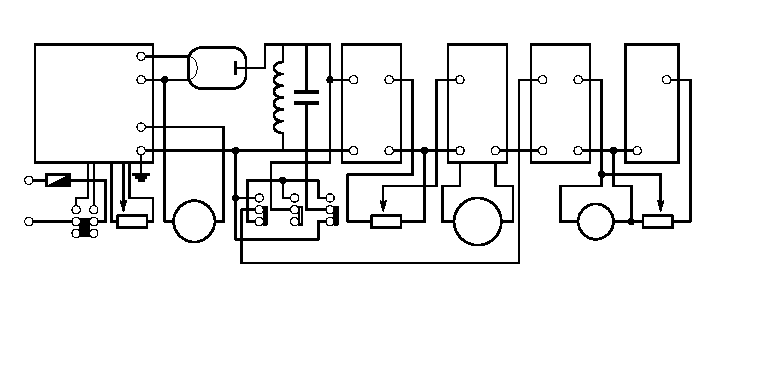
\includegraphics[width=\textwidth]{2_7_2}
	\caption{Блок-схема установки для измерения дробового шума. Внизу изображена нижняя часть передней панели с ручками и кнопками управления}
	\figmark{exp Schottky noise}
\end{figure}
%\fcpic[1]{2_7_2}{Блок-схема установки для измерения дробового шума. Внизу изображена нижняя часть передней панели с ручками и кнопками управления}{2}

Сила анодного тока шумового диода в режиме насыщения определяется эмиссией (а значит, температурой) его катода. Анодный
ток $I_{\text{а}}$ измеряется миллиамперметром и регулируется потенциометром $R_{\text{а}}$, ручка которого на панели прибора обозначена
<<$R_{\text{а}}$>>. Чувствительность измерительной схемы регулируется делителем напряжения $R_{\text{д}}$, расположенным между усилителем
и квадратичным детектором. Его ручка на панели обозначена <<$R_{\text{д}}$>>. На выходе квадратичного детектора установлен
микроамперметр. Отклонение стрелки микроамперметра пропорционально квадрату напряжения на входе детектора, поэтому он
пригоден для измерения переменных напряжений. Таким образом, показания микроамперметра пропорциональны квадрату шумового
напряжения, причём коэффициент пропорциональности зависит от положения реостата $R_{\text{д}}$ и, вообще говоря, неизвестен.
Поэтому при измерениях экспериментатор замечает показание микроамперметра, а затем вместо сигнала с колебательного
контура подаёт на вход усилителя калибровочный сигнал с настроенного на ту же частоту генератора. Этот сигнал измеряется
вольтметром (обозначение <<$U_{\text{г}}$>> на панели) и ослабляется в точно известное число раз прецизионным аттенюатором. При
измерениях напряжение на генераторе подбирается так, чтобы стрелка микроамперметра вернулась к отмеченному делению. В
этом случае напряжение шумов равно известному напряжению, подаваемому на усилитель с аттенюатора. Делитель $R_{\text{д}}$ во
время этой процедуры, конечно, нельзя трогать.

Генератор используется не только для калибровки квадратичного детектора, но и для измерения добротности контура.
Измерения производятся по методу $Q$-метра. Включим в контур генератор~Г (настроенный на собственную частоту контура),
как это изображено на рис.~\figref{scheme Q}. Выходное напряжение генератора $U_{\text{г}}$ целиком падает на активном сопротивлении контура $R$.
Поэтому $U_{\text{г}}=IR$, где $I$~---~ток в контуре. Найдём теперь напряжение $U_{\text{к}}$, подаваемое на усилитель и измеряемое
квадратичным детектором:
\begin{equation*}
U_{\text{к}}=U_{\text{г}}-\frac{I}{i\omega C}=U_{\text{г}}-\frac{U_{\text{г}}}{i\omega RC}\approx\frac{iU_{\text{г}}}{\omega RC}.
\end{equation*}
При написании последнего равенства считалось, что контур обладает высокой добротностью, $Q=1/\omega RC\gg1$. Заменяя $1/\omega
RC$ через добротность контура, найдём
\begin{equation}
	\eqmark{2.7.13}
	Q=\frac{|U_{\text{к}}|}{|U_{\text{г}}|}.
\end{equation}
%\todo[author=Tiffani]{Сделать нормальный рисунок.}
\begin{figure}[h!]
	\pic{0.9\textwidth}{2_7_3}
	%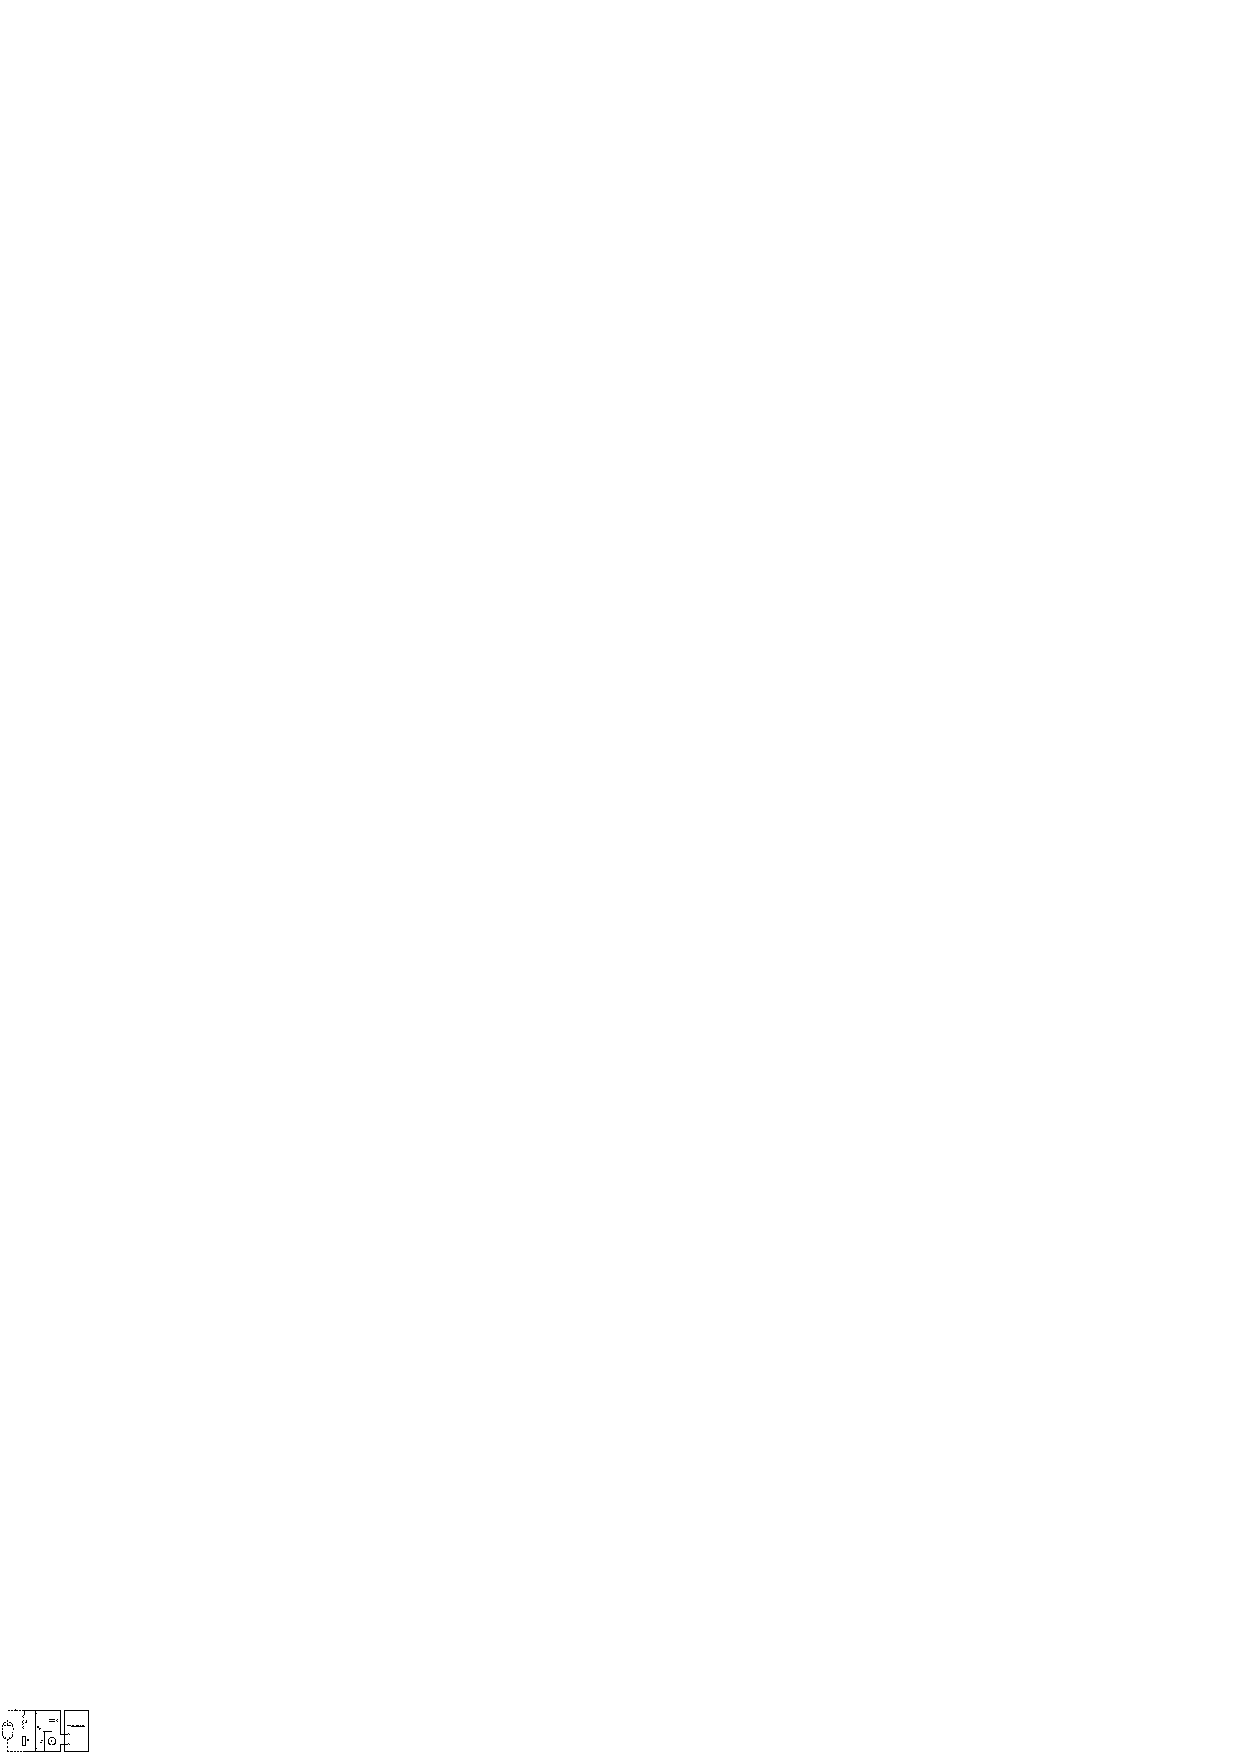
\includegraphics[width=\textwidth]{2_7_3}
	\caption{Схема для измерения добротности колебательного контура}
	\figmark{scheme Q}
\end{figure}
%\rpic{55mm}{2_7_3}{\cct Схема для измерения добротности колебательного контура}{3}

Итак, для измерения добротности контура нужно сравнить напряжение на генераторе с напряжением на катушке самоиндукции.
Напряжение на генераторе $U_{\text{г}}$ измеряется вольтметром генератора (рис.~\figref{exp Schottky noise}). Измерение напряжения на катушке самоиндукции
не так просто.

При измерении напряжения $U_{\text{к}}$, создаваемого генератором на катушке самоиндукции, необходимо учитывать и шумовое
напряжение $U_{\text{ш}}$, имеющееся на катушке. Это напряжение при измерениях продолжает возбуждаться диодом, так как при
измерениях добротности контура диод находится в рабочем режиме. Отключить диод при измерении нельзя, поскольку
добротность контура от этого заметно изменится: при измерениях шума контур шунтирован диодом, что снижает его
добротность; в этом положении и должна измеряться добротность контура. При включении генератора в контур на вход
усилителя поступает не $U_{\text{к}}$, как показано на рис.~\figref{scheme Q}, и не $U_{\text{ш}}$, а их сумма. При этом ток детектора $I_{\text{д}}$ пропорционален
$\langle (U_{\text{ш}}+U_{\text{к}})^2\rangle$. Сдвиг фаз между колебаниями $U_{\text{ш}}$ и $U_{\text{к}}$ непрерывно изменяется. Поэтому
\begin{equation*}
I_{\text{д}}\propto\langle (U_{\text{ш}}+U_{\text{к}})^2\rangle=\langle U_{\text{ш}}^2\rangle+2\langle U_{\text{ш}}U_{\text{к}}\rangle+\langle U_{\text{к}}^2\rangle=\langle U_{\text{ш}}^2\rangle+\langle U_{\text{к}}^2\rangle,
\end{equation*}
в то время как до включения генератора ток детектора $I_{\text{д}}$ был пропорционален $U_{\text{ш}}^2$.

Таким образом, $U_{\text{к}}^2$ пропорционально \important{приращению} тока квадратичного детектора, происходящему при включении
напряжения $U_{\text{г}}$. Чтобы подставить это приращение в формулу \eqref{2.7.13}, оно должно быть пересчитано в напряжение
генератора. Это делается следующим образом. Нужно заметить показание квадратичного детектора при нулевом напряжении на
выходе генератора. Затем нужно установить на выходе генератора некоторое напряжение $U_{\text{г}}$ и зафиксировать приращение
тока детектора $\Delta I_{\text{д}}$, вызванное напряжением генератора. После этого вместо колебательного контура на вход усилителя
следует подключить генератор с аттенюатором. Сигнал с генератора и положение аттенюатора нужно подобрать таким образом,
чтобы показание микроамперметра было равно измеренному ранее приращению $\Delta I_{\text{д}}$. Показание вольтметра генератора равно
искомому напряжению $U_{\text{к}}$.

\begin{lab:task}
В работе предлагается, измерив напряжение шумов, раскачивающих колебательный контур, и определив добротность этого
контура, рассчитать заряд электрона.

%\todo[author=Tiffani]{Сделать нормальный рисунок. Этот даже не отображается}
\begin{figure}[h!]
	\pic{0.9\textwidth}{2_7_4}
	\caption{Схема установки для измерения напряжения шума}
	\figmark{scheme U noise}
\end{figure}
	\begin{enumerate}
		\tasksection{Проверка квадратичности детектора}

	\item Включите питание стенда (кнопка <<Сеть>>).

	\item Убедитесь в том, что выпрямительная схема с полупроводниковыми диодами действительно имеет квадратичную
характеристику. Для этого включите стенд в режим измерения напряжения генератора (кнопка <<$U_{\text{г}}$>>). Установите
максимальную  чувствительность квадратичного детектора (регулятор~$R_{\text{д}}$) и подберите предел измерений для вольтметра
(кнопка <<100>> или <<300>>~мкВ аттенюатора). Изменяя выходное напряжение генератора с помощью регулятора напряжения
генератора $R_{\text{г}}$, снимите зависимость тока квадратичного детектора $I_{\text{д}}$ от входного напряжения усилителя~$U_{\text{г}}$.

		\tasksection{Измерение напряжения шума}
 
	\item Включите режим измерения шума (кнопка <<$U_{\text{ш}}$>>). Электрическая схема для этого случая показана на рис.~\figref{scheme U noise}.

	\item Установите анодный ток шумового диода $I_{\text{а}}=1$~мА, изменяя регулятором $R_{\text{А}}$ напряжение накала диода.

С помощью регулятора $R_{\text{д}}$ подберите чувствительность квадратичного детектора так, чтобы стрелка микроамперметра
отклонялась на б\'ольшую часть шкалы. Отметьте значение шумового тока~$I_{\text{д}}$.

Для пересчёта отклика детектора на шум в единицы напряжения вместо шумового диода подключите к усилителю генератор
напряжений (кнопка~<<$U_{\text{г}}$>>). Измерительная схема приведена на рис.~\figref{scheme U generator}.

%\todo[author=Tiffani]{Сделать нормальный рисунок. Этот даже не отображается}
\begin{figure}[h!]
	\pic{0.9\textwidth}{2_7_5}
	\caption{Схема установки для измерения напряжения на генераторе}
	\figmark{scheme U generator}
\end{figure}

С помощью регулятора $R_{\text{г}}$ и аттенюатора (пределы <<30>>, <<100>> или <<300>>~мкВ) установите \important{то же значение
тока}~$I_{\text{д}}$, которое было выбрано в режиме измерения шума. Регулятор $R_{\text{д}}$ во время этой процедуры, конечно, трогать
нельзя. Отсчитанное по вольтметру с аттенюатором напряжение~$U_{\text{эфф}}$ равно корню квадратному из среднего квадрата
напряжения шумов.

			\tasksection{Измерение добротности контура}

	\item При том же анодном токе диода переключите аттенюатор в положение <<1>> или <<3>>~мкВ. Установите режим измерения
напряжения на контуре при его последовательном возбуждении (кнопка~<<$U_{\text{к}}$>>). При нулевом напряжении на вольтметре
подберите чувствительность детектора: регулятором $R_{\text{д}}$ установите стрелку микроамперметра детектора на любое целое
деление. Измерьте \important{приращение} тока детектора $\Delta I_{\text{д}}$ при изменении напряжения генератора от нуля до любого
напряжения~$V_1$.

Затем включите режим измерения напряжения на генераторе (кнопка~<<$U_{\text{г}}$>>) и регулятором $R_{\text{г}}$ подберите напряжение
$V_2$, при котором ток квадратичного детектора равен \important{приращению} $\Delta I_{\text{д}}$ в режиме измерения сигнала с~контура.
Добротность контура равна $Q=V_2/V_1$.

	\item Повторите измерения по пунктам 2~--~3 ещё 5~--~6 раз при том же анодном токе (можно при другой
чувствительности детектора).

	\item Проведите измерения по пунктам 2~--~4 при других значениях анодного тока в интервале 1~--~4~мА.

	\item Запишите значения ёмкости и резонансной частоты колебательного контура, указанные на установке.
	
\end{enumerate}

\begin{enumerate}
		    \tasksection{Обработка результатов}

	\item Постройте график зависимости $I_{\text{д}}=f(U^2_{\text{г}})$ для проверки характера детектирования.

	\item Вычислите среднюю величину заряда электрона для каждого значения тока анода. Представьте результаты в виде таблицы.

%\bigskip
\begin{center}
\begin{tabular}{|c|c|c|c|c|}
\hline $\;I_{\text{а}}$,~мА&$\;U_{\text{эфф}}$,~мкВ&$\quad\langle Q\rangle\quad$&$e~$, Кл&$\langle e\rangle\pm\Delta e$\\\hline\hline
 & & & &\\
 & & & &\\
 & & & &\\
 & & & &\\
\hline
\end{tabular}
\end{center}

	\item Определите заряд электрона, используя все полученные результаты, и оцените погрешность. Сравните полученное значение
с табличным.
	\end{enumerate}
\end{lab:task}
\todo[author=Tiffani]{Нет вопросов к лабораторной.}

\begin{lab:literature}
	\item \emph{Власов~В.Ф.} Электронные и ионные приборы.~--- М.:~Связьиздат, 1960, \S~13.5.

	\item \emph{Рытов~С.М.} Введение в статистическую радиофизику.~--- М.:~Наука, 1976, \S~5.
\end{lab:literature}